\documentclass[
portrait,
custom
]{sciposter}
\renewcommand{\sectionsize}{\large}
\renewcommand{\titlesize}{\Huge}
\graphicspath{{img/}}

\usepackage{multicol}
\setlength\columnseprule{0pt}
\setlength{\columnsep}{2.5pc}

\usepackage{tikz}
\usetikzlibrary{mindmap}

\usepackage{soul}

\usepackage{amssymb}            % \blacksquare
\usepackage{amsmath}            % \text

\usepackage{tabularx}
\newcolumntype{C}{>{\centering\arraybackslash}X}
\newcolumntype{R}{>{\raggedleft\arraybackslash}X}
% Vertically center within row https://tex.stackexchange.com/a/343329
\renewcommand\tabularxcolumn[1]{m{#1}}
\usepackage{booktabs}
\usepackage{multirow}

\usepackage[
abbreviate=true,
bibencoding=utf8,
minnames=2,
maxbibnames=99,
sorting=none,
style=vancouver,
citestyle=numeric-comp
]{biblatex}
% The vancouver citation style is based on NLM per
% https://tex.stackexchange.com/a/371433
\addbibresource{references.bib}
\renewcommand*{\bibfont}{\footnotesize\selectfont}

\title{GPUs for massively parallel mechanistic modeling}
\renewcommand{\thefootnote}{\fnsymbol{footnote}}
\author{Pariksheet Nanda\textsuperscript{\footnotemark[2]}, %
  Elijah MacCarthy\textsuperscript{\footnotemark[3]}}
\institute{\textsuperscript{\footnotemark[2]}University of Pittsburgh, %
  \textsuperscript{\footnotemark[3]}Oak Ridge National Laboratory}
\norightlogo{}
\leftlogo[1.4]{logo-pitt}

\begin{document}
\maketitle

\begin{multicols}{2}

  \section*{Purpose of the course}
  Graphical Processing Units (GPUs) %
  are integrated into the core architecture %
  of the world's fastest supercomputers %
  that solve the most computationally difficult, %
  mechanistic scientific problems.
  %
  An 8~year, \$1.8~billion effort %
  called the Exascale Computing Project (ECP) %
  involving 2,800 scientists and engineers %
  recently finished modernizing %
  the underlying scientific numerical software %
  to efficiently use this new generation of machines.
  \medskip
  
  Computing facilities grant access at no cost %
  to these GPU-accelerated%
  \supercite{%
    carter_2014,%
    beckingsale_2019,%
    reinders_2023%
  } machines %
  only to research software engineers and scientists who demonstrate that %
  their computations scale %
  to efficiently use multiple GPUs across many computer servers / nodes.
  %
  Therefore, %
  it is imperative to teach %
  the data parallel software development skills, %
  appropriate domain science methods, and %
  sustainable software practices %
  to enable large scale, GPU-centric computational research.
  \medskip
  
  This course trains graduate researchers %
  with ECP-level skills in high performance computing (HPC), %
  using research software engineer (RSE) rigor, %
  and HPC-relevant domain scientific methods.
  %
  Discussion and feedback on this poster from the community %
  can help make this course a success and %
  support similar hands-on learning and teaching endeavors.

  \section*{Course overview}
  \begin{figure}
    \begin{minipage}[c]{.31\linewidth}
      \caption{\emph{\textbf{Course topics.}
          %
          The topics covered in this planned course %
          are organized into the categories of the %
          \textcolor{red!80!black}{$\blacksquare$}~capstone project,
          \textcolor{orange!90!black}{$\blacksquare$}~performance optimization, %
          \textcolor{blue!80!black}{$\blacksquare$}~software development, %
          \textcolor{green!50!black}{$\blacksquare$}~domain science methods, and %
          \textcolor{black!60}{$\blacksquare$}~cluster administration.
          %
          Each leaf node more-or-less corresponds to %
          a single classroom session.}}
    \end{minipage}
    %\hfill
    \begin{minipage}[c]{.69\linewidth}
      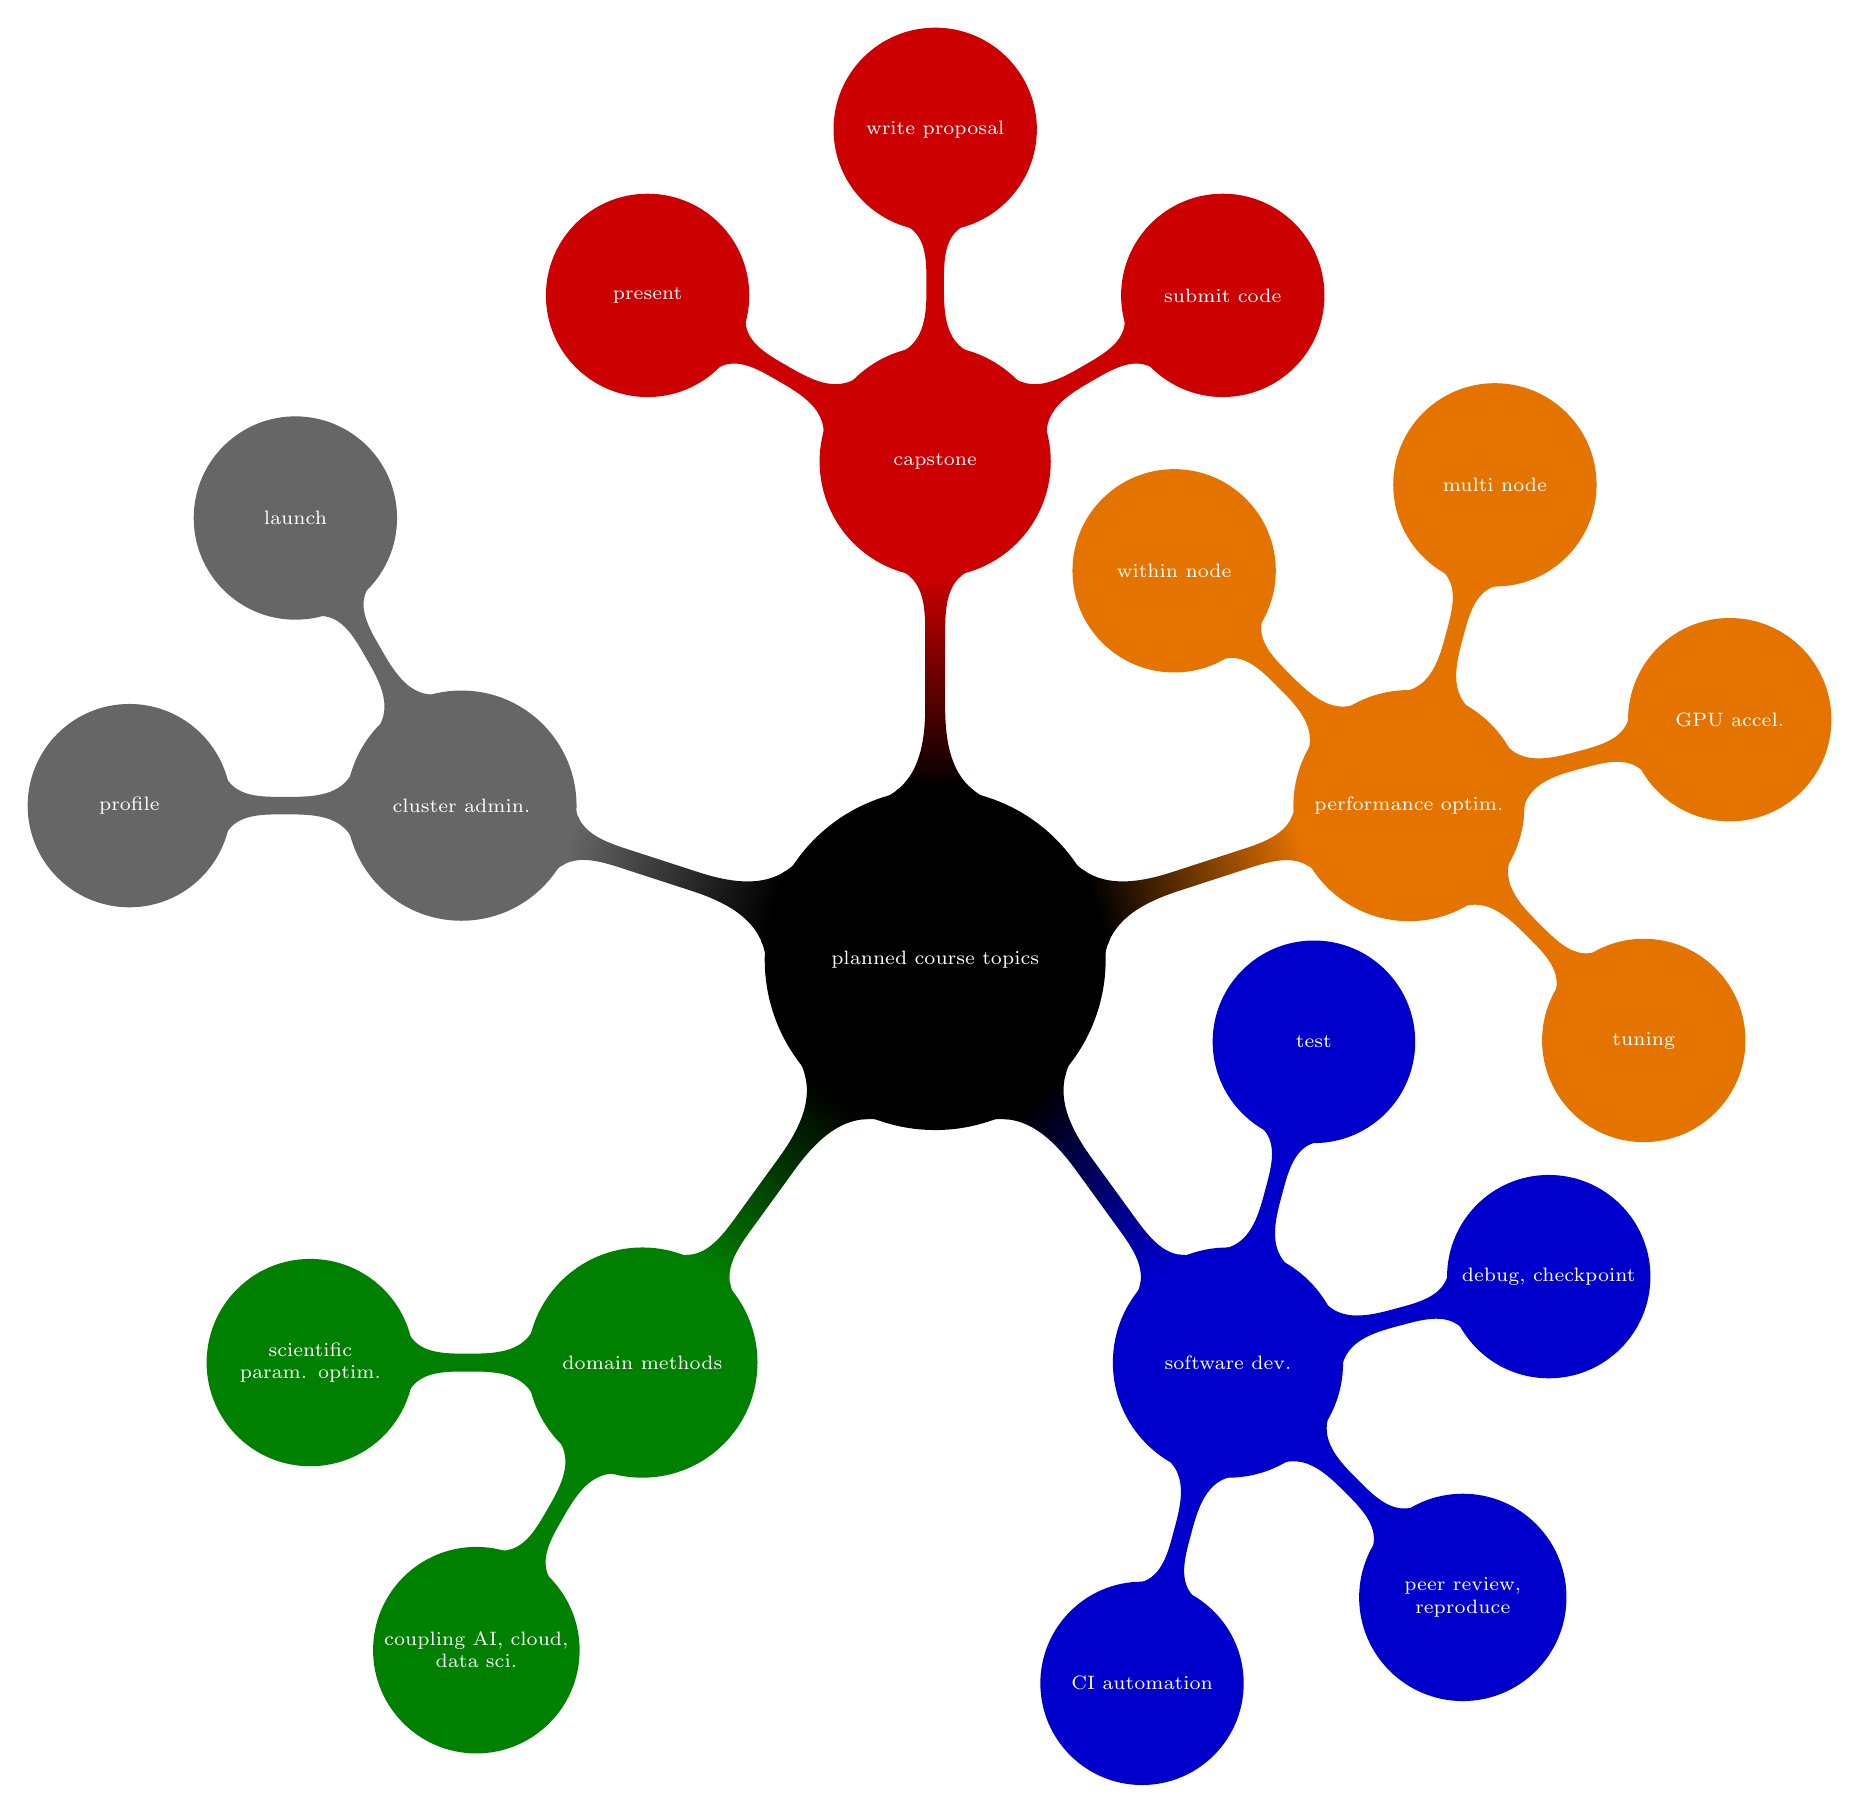
\begin{tikzpicture}[
        root concept/.style={
          text width = 120pt,
        },
        level 1 concept/.style={
          text width = 80pt,
          level distance = 180,
        },
        level 2 concept/.append style={
          text width = 70pt,
          level distance = 120,
        },
        every concept/.append style={
          font = \scriptsize,
        },
        mindmap,
        ]
        \path
        node [concept, concept color=black, text=white] {planned course topics}
        child [grow=90, concept color=red!80!black, text=white] {
          node [concept] {capstone}
          [clockwise from=150]
          child { node [concept] {present} }
          child { node [concept] {write proposal} }
          child { node [concept] {submit code} }
        }
        child [grow=18, concept color=orange!90!black, text=white] {
          node [concept] {performance optim.}
          [clockwise from=135]
          child { node [concept] {within node} }
          child { node [concept] {multi node} }
          child { node [concept] {GPU accel.} }
          child { node [concept] {tuning} }
        }
        child [grow=306, concept color=blue!80!black, text=white] {
          node [concept] {software dev.}
          [clockwise from=75]
          child { node [concept] {test} }
          child { node [concept] {debug, checkpoint} }
          child { node [concept] {peer review, reproduce} }
          child { node [concept] {CI automation} }
        }
        child [grow=234, concept color=green!50!black, text=white] {
          node [concept] {domain methods}
          [counterclockwise from=180]
          child { node [concept] {scientific param. optim.} }
          child { node [concept] {coupling AI,~cloud, data sci.} }
        }
        child [grow=162, concept color=black!60, text=white] {
          node [concept] {cluster admin.}
          [counterclockwise from=120]
          child { node [concept] {launch} }
          child { node [concept] {profile} }
        };
      \end{tikzpicture}
    \end{minipage}
  \end{figure}

  \begin{table}
    \caption{\emph{\textbf{High-level comparison of topics.}
        %
        Comparison of this course with the %
        2024 Argonne Training Program on Extreme-Scale Computing (ATPESC'24) %
        and the 2025 Lawrence Livermore National Laboratory %
        High Performance Computing Innovation Center (HPC-IC'25) %
        tutorial series.
      }}
    \begin{tabularx}{\linewidth}{%
      >{\hsize=.15\hsize\linewidth=\hsize}X %
      >{\hsize=.34\hsize\linewidth=\hsize}R %
      >{\hsize=.16\hsize\linewidth=\hsize}C %
      >{\hsize=.16\hsize\linewidth=\hsize}C %
      >{\hsize=.16\hsize\linewidth=\hsize}C}
      \toprule
      Category
      & Topic
      & This Course & ATPESC'24 & HPC-IC'25\\
      \midrule
      \multirow{3}{\hsize}{Performance optimization}
      & Within node
      & \checkmark & \checkmark & $\times$\\
      & Multi-node
      & \checkmark & \checkmark & \checkmark\\
      & \mbox{GPU performance\ldots} \ldots{}portability
      & \checkmark & \checkmark & \checkmark\\
      \midrule
      \multirow{7}{\hsize}{Software development}
      & Unit and performance testing
      & \checkmark & \checkmark & \checkmark\\
      & Parallel debugging
      & \checkmark & \checkmark & $\times$\\
      & Checkpointing
      & \checkmark & $\times$ & $\times$\\
      & Unit testing
      & \checkmark & \checkmark & $\times$\\
      & Continuous integration
      & \checkmark & $\times$ & \checkmark\\
      & Code peer review
      & \checkmark & $\times$ & $\times$\\
      & Reproducibility
      & \checkmark & \checkmark & \checkmark\\
      \midrule
      \multirow{-1.5}{\hsize}{Domain science methods}
      & \mbox{Gradient-free optimization\ldots{}} \mbox{\ldots{}of model parameters}
      & \checkmark & \checkmark & \checkmark\\
      & Coupling AI, cloud, data sci.
      & \checkmark & $\times$ & \checkmark\\
      \midrule
      Sysadmin
      & Cluster launch
      & \checkmark & $\times$ & \checkmark\\
      \bottomrule
    \end{tabularx}
  \end{table}

  \section*{Science gateways resources}
  \begin{description}
  \item[JetStream2-GPU:] non-virtual multi-GPU A100 nodes (g3.2xl)
    \begin{itemize}
    \item Shared between small groups of 4 students.
    \item For early project development and exercises.
    \item A100 supports FP64 for capstone projects that need it.
    \item Efficient multi-GPU use is a course objective.
    \item g3.2xl is the multi-GPU A100 with the most availability.
    \end{itemize}
  \item[ACCESS CI:] Bridges-2 GPU HPC Allocation
    \begin{itemize}
    \item For cluster exercises and scaling.
    \item Interactive nodes with backfill scheduling and short walltime %
    for the classroom use.
    \end{itemize}
  \item[GitHub Workflows:] Trainee repositories for assignments and projects
    \begin{itemize}
    \item Projects in private git repositories shared with the instructor.
    \item Assignments will be partially checked using GitHub workflows.
    \item Progress on capstone projects will be monitored from git repositories.
    \end{itemize}
  \end{description}

  \section*{Syllabus changes guided by mentors, hosts \& guest speakers}
  \begin{multicols}{2}
    \begin{enumerate}
    \item \ul{Consolidated course topics} %
      to allow for more focus on domain science methods %
      in keeping with the course title.
    \item \ul{Added an AI policy} %
      that requires a bibliography %
      citing AI service names with versions, prompts, and output.
    \item Moved non-capstone homework assignments to %
      \ul{classroom hands-on to avoid over-reliance on AI support} %
      while trainees are still developing expertise.
    \item \ul{Increased accessibility} %
      to less experienced C/C++ programmers %
      by recommending self-guided, open access textbooks %
      from \emph{The Art of HPC: Volume 3}.
    \item \ul{Added objective of numerical correctness} %
      but limited goal to unit tests, performance test, and CI %
      instead of considering formal methods.
    \item \ul{Decided on a checkpointing library} %
      written in C/C++ %
      both to teach in the course %
      and for wider use in student capstone projects.
    \item \ul{Added network communication exercise} %
      using the LAMMPS exercise developed at Temple University.
    \item \ul{Added profiling exercises} %
      from, Cornell University %
      and the University of Michigan.
    \item Trainees will \ul{write C/C++ code using VS Code} %
      with SSH tunnels to JetStream2 virtual machines %
      with a fallback of OpenVSCode Server web interface %
      for classroom instruction.
    \item The target audience is now \ul{graduate students} %
      with existing projects or pilot projects.
    \end{enumerate}
  \end{multicols}

  \section*{Acknowledgments}
  This course revision was supported %
  by the FacultyHack hosts and mentors %
  under NSF award 2231406; %
  however no NSF financial support was provided %
  because this is a new course being piloted %
  and not an existing course begin revised.
  \medskip

  Developing HPC expertise was supported by the 2024 %
  Argonne Training Program on Extreme-Scale Computing (ATPESC) %
  by the Department of Energy, %
  Office of Science, %
  Advanced Scientific Computing Research (ASCR) program.
  %
  Additional HPC expertise was supported by the 2025 Tutorials from the %
  High Performance Computing Innovation Center (HPC-IC) at %
  Lawrence Livermore National Laboratory.
  \medskip

  The uncertainty quantification methodologies %
  for agent-based, mechanistic, multiscale modeling %
  and similar gradient-free approaches%
  \supercite{%
    nanda_2023,%
    aguiar_2024%
  } % 
  were supported by NIH grant R01~AI50684.

  \section*{References}
  {
    % Recalculate \columnsep instead of using the large \columnsep
    % from the main document.
    \setlength{\columnsep}{1.5pc}
    \begin{multicols}{2}
      \printbibliography[heading=none]{}
    \end{multicols}
  }

\end{multicols}

\end{document}
